\chapter{Introduction}
\label{sec:introduction-chapter}

\section{The Capacitated Vehicle Routing Problem}
\label{sec:intro-cvrp-problem}
The \textit{Capacitated Vehicle Routing Problem} (\textbf{CVRP}), first presented in \textcite{dantzig1959}
under the name of "truck dispatching problem",
is one of the most studied combinatorial optimization routing problems.
The CVRP is an NP-hard (in the strong sense) problem
that can be considered a generalization of the well-known Travelling Salesman Problem (TSP).
The TSP \parencite{flood1956}
is an NP-hard \parencite{garey1976planar} ubiquitous combinatorial optimization problem in the operations research field,
that asks for the determination of a Hamiltonian circuit of minimum cost
\parencite{croes1958, laporte1992,johnson1997,applegate2006,gutin2006,hoffman2013}.
The CVRP can be defined verbally as finding an optimal route for a transportation/distribution/delivery problem
starting from a common point called the depot,
where a homogeneous fleet composed of a fixed number of trucks, subject to capacity constraints,
need to serve customer demands of a single good (i.e. delivery of gasoline to gas stations).
Given as input: a weighted graph representing the road network,
the customer demands and the vehicle capacity,
the problem consists in determining a set of non-oriented routes, one for each vehicle,
of minimal overall travel distance starting and ending at the depot.
The set of routes needs to serve all the customers in the road network exactly once
while satisfying the vehicle capacity bound \parencite{toth2014}.
A diagram showing an example of a CVRP problem along with its optimal solution
is provided in \Cref{fig:cvrp-optimal-solution-example}.

\begin{figure}[t]
	\centering
	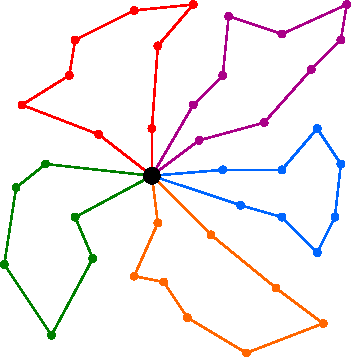
\includegraphics[width=12cm]{Imgs/P-n40-k5-solution.out.cropped.pdf}
	\caption{An illustration of an optimal CVRP solution (instance named P-n40-k5).
		There are $39$ customers to serve and $5$ trucks with a capacity of $140$ units each.
		Each color in the picture represents a different route that each truck has taken.
		Instead, the colored dots represent the customers served by each truck on its route.
		The customer demands are not depicted for the sake of clarity.
		The larger black dot in the center represents the depot where each route must begin and end.
		Credits: \url{http://vrp.galgos.inf.puc-rio.br/index.php/en/plotted-instances?data=P-n40-k5}.
	}
	\label{fig:cvrp-optimal-solution-example}
\end{figure}

Investigating effective CVRP solution methods may result in
significant real-world economic savings for the management
of the provision of goods or services in a distribution system.
Optimal delivery planning can reduce the overall transportation, goods costs,
and waiting time experienced by the customers.
As a result, researching efficient exact algorithms and mathematical models
for solving and describing real-world distribution problems
becomes critical for the operational management
of a cost-effective planning process \parencite{toth2002,toth2014}.

The CVRP is part of a larger class of problems known as the Vehicle Routing Problems (VRPs).
There are many variations of VRPs proposed in the literature, including
the \textit{Vehicle Routing Problem with Time Windows} (VRPTW) \parencite{schrage1981}
and many others.
The vehicles in the VRPTW are subject to capacity constraints
and must serve each customer within an allocated time window slot.
Nonetheless, CVRP is the simplest VRP variant to describe,
and to this day, it remains the most central and studied routing problem.
For a comprehensive taxonomy of the many VRP variants, refer to \textcite{eksioglu2009, braekers2016}.

While effective (meta-)heuristic algorithms have been proposed and applied
successfully to many VRP variants to obtain good-enough solutions
in reduced computation time,
the focus of this thesis is on exact algorithms for solving the CVRP.

We can find major contributions employing heuristics for the VRP, among others, in
\textcite{clarke1964, desrochers1989matching, paessens1988savings, foster1976integer}.
Meta-heuristics approaches for the VRP can be found in
\textcite{gendreau1994tabu, cordeau2012parallel, toth2003granular, li2005very, pisinger2007, kytojoki2007efficient, nagata2009,vidal2012, subramanian2013},
just to name a few.

For a more comprehensive survey on (meta-)heuristics for the VRP, refer to
\textcite{golden1998impact,gendreau2002metaheuristics,gendreau2008,laporte2014chapter,elshaer2020taxonomic}.

Exact algorithms are typically slower than (meta-)heuristics, but given
enough computation time, they can produce a proven optimal solution.
They accomplish this by closing the objective function's primal-dual bound gap.

\medskip

We strongly recommend the book  "\citetitle{toth2014}" of \textcite{toth2014}
for a comprehensive overview/survey on the CVRP and VRPTW problems,
as well as other common VRP variants.
This book served as a good reference and was instrumental in laying the groundwork
for the first chapters of this thesis.
We also gathered additional information from other VRP surveys in the works of
\textcite{cordeau2007, baldacci2012, caceres-cruz2015, costa2019}.

\section{Thesis Contributions}
\label{sec:intro-thesis-contributions}

Modern CVRP solvers are typically developed and tested on test sets comprised of historical benchmark instances.
The principal historical test instances used to evaluate the performance of the scientific contributions have been divided into families.
Each family is represented by a single upper case letter.
The major CVRP test sets proposed by the operations research community over the years are summarized here:
\begin{itemize}
	\setlength{\itemsep}{0pt}
	\setlength{\parskip}{0pt}

	\item The set \texttt{E} is proposed in\textcite{dantzig1959, christofides1969, gaskell1967bases, gillett1974heuristic}.
	      The majority of the \texttt{E} test instances were generated at random, while the remainder lack description on their origin.
	\item The set \texttt{M} was proposed in \textcite{christofides1979vehicle} and was obtained by aggregating instances from \texttt{E} set.
	\item The set \texttt{F} was presented in \textcite{fisher1994} and was obtained from an actual distribution problem of groceries in the city of Ontario.
	\item The sets \texttt{A}, \texttt{B} and \texttt{P} were all proposed in \textcite{augerat1995}.
	      The sets \texttt{A}, \texttt{B} were generated at random, while the set \texttt{P} was generated from sets \texttt{A}, \texttt{B} and \texttt{E} by changing the capacities.
\end{itemize}
These historical benchmark instances bear little resemblance to real-world distribution problems.
They are either too homogeneous or too artificial while not covering the key characteristics found in contemporary real-world distribution problems.
The historical instances presented in the literature are typically characterized by stringent vehicle capacities, which give rise to optimal solutions characterized by short routes each visiting few customers.
Instead, real-world contemporary distribution problems are characterized by much longer routes since the vehicle capacity is rarely the bottleneck in practice.
Despite \textcite{uchoa2017} proposed \texttt{X} test-set, a broader and trendier common denominator of diverse instances for the CVRP, the historical test instances were (and continue to be) the primary central test-bed for comparing and assessing the performance of CVRP contributions.

The \textit{labeling algorithm} is a dynamic programming-based algorithm used to solve the pricing sub-problem induced from \textit{Column Generation} (CG) schemes applied to the VRP.
We will delve into these topics in greater detail in \cref{sec:branch-and-price}.
The labeling algorithm is a crucial component of the contemporary state-of-the-art CVRP solvers \parencite{gutierrez-jarpa2010, archetti2011, bettinelli2011, contardo2014, contardo2015, pecin2017new, pecin2017improved, pessoa2020generic}.
As we shall discuss later, the performance of the labeling algorithm degrades as the vehicle capacity increases, see discussion in \cref{sec:solving-the-pricing-problem}.

In this thesis, we investigate the feasibility and competitiveness of a branch-and-cut algorithm implemented through a commercial MIP software package for solving the pricing problem.
The goal is to empirically compare the performance of the proposed branch-and-cut framework against the state-of-the-art labeling algorithm while empirically measuring how the two frameworks behave as the lengths of the route they need to generate increases.

\Textcite{jepsen2014} proposed a branch-and-cut framework for the CPTP and tested it in the context of pricing for the CVRP.
\Textcite{jepsen2014} demonstrated that, while the labeling algorithm was much faster in many instances, the BAC framework exhibited better performance for some bulkier cases.
See later discussion in \cref{sec:bac-approaches-for-the-pricing-problem}.
They demonstrated that further research on BAC-pricers could yield approaches that could supplement the traditional pricing labeling algorithm.
We revisit the work of \citeauthor{jepsen2014} in this thesis.
We test whether recent advancements in MIP optimizers have made them competitive at solving the pricing problem or whether modern dynamic programming algorithms have rendered BAC approaches completely obsolete.

\section{Outline}
\label{sec:intro-outline}

This section provides an overview of the work's contents.
The thesis' contents can be divided into three major portions, which we will list here.

The first portion provides introductory technical material
regarding the CVRP and contemporary resolution methods for this problem.
\Cref{sec:cvrp-mathematical-formulations} formalizes the CVRP
through multiple mathematically rigorous integer programming models.
\Cref{sec:intro-literature-review} summarizes the notable contributions
of the operations research practitioners regarding CVRP's exact approaches.
The branch-and-price (BPC) algorithm, column generation,
and the pricing sub-problem are presented in \cref{sec:branch-and-price}.
The most recent exact algorithms for solving routing problems are all BPC-based.
Recent research has empirically demonstrated that BPC algorithms
perform admirably in the routing problem domain.

In the second part of the thesis,
we will go over the pricing sub-problem in greater detail,
as well as our branch-and-cut (BAC) pricer implementation.
The pricing sub-problem is a combinatorial optimization problem
that arises when a CVRP is solved using a BPC approach.
\Cref{sec:the-pricing-problem} introduces and discusses the pricing sub-problem
through multiple mathematically rigorous integer programming models.
The implementation details of our proposed branch-and-cut pricer
are presented in \cref{sec:implementation-chapter}.

The third part of the thesis evaluates the competitiveness of the proposed BAC framework
in solving the pricing sub-problem.
We evaluate its performance and compare it to modern cutting-edge solutions.
In \cref{sec:results} we present the evaluation setup, we list the instances employed,
and finally, we show the empirical results along with a discussion.
Finally, in \cref{sec:conclusions} we summarize the work, review the results
and offer helpful tips while discussing potential implementation improvements.
